% mycsrf 'for beeing included' snippet template
%
% (c) Karsten Reincke, Frankfurt a.M. 2012, ff.
%
% This text is licensed under the Creative Commons Attribution 3.0 Germany
% License (http://creativecommons.org/licenses/by/3.0/de/): Feel free to share
% (to copy, distribute and transmit) or to remix (to adapt) it, if you respect
% how you must attribute the work in the manner specified by the author(s):
% \newline
% In an internet based reuse please link the reused parts to mycsrf.fodina.de
% and mention the original author Karsten Reincke in a suitable manner. In a
% paper-like reuse please insert a short hint to mycsrf.fodina.de and to the
% original author, Karsten Reincke, into your preface. For normal quotations
% please use the scientific standard to cite
%


%% use all entries of the bibliography

\subsubsection{EasyABC}

Seine Repositoryseite sagt von \acc{EasyABC}, es sei in Python geschriebenes
Notensatzprogramm, das für die graphische Darstellung auf das
Kompatibilitätsframework \acc{WxWidgets} zurückgreife.\footcite[vgl.][\nopage
wp]{EasyAbc2017a}. Die letzte Version stammt vom Mai
2018.\footcite[vgl.][\nopage wp]{EasyAbc2017c} Das Open Source Projekt pflegt
außerdem eine Projekthomepage, die Installationsoptionen
auflistet.\footcite[vgl.][\nopage wp]{EasyAbc2017b}. Neben diesen beiden
Anlaufpunkten exisitert noch die (veraltete) Homepage des ursprünglichen
Programmierers\footcite[vgl.][\nopage wp]{Liberg2015a}.

(Aktuelle) Distributionen werden \acc{EasyABC} eher nicht mit
anbieten.\footnote{Ubuntu 18.04 jedenfalls offeriert kein entsprechendes Paket.}
Denn -- laut \acc{EasyABC} Installationsanleitung -- gäbe es intendiert keine
entsprechenden Installations- oder Binärpakete: \acc{EasyABC} solle per Shell --
über den Befehl \texttt{python easy\_abc.py} -- direkt aus dem heruntergeladenen
Ordner mit den Softwarequellen gestartet werden, damit das Programm all seine
Resourcen finde.\footnote{Das Quellpaket enthält eine Linuxanleitung (=
\texttt{using\_EasyABC\_in\_Windows.txt}) und eine Windowsanleitung (=
\texttt{using\_EasyABC\_in\_Linux.txt}), die jeweils auflisten welche
Zusatzpakete installiert sein müssen, bevor man \acc{EasyABC} erfolgreich
starten kann. Ubuntu 18.04 Nutzer müssen bei der Abarbeitung der Liste
aufpassen: Python3 ist Distributionsstandard, während Python2.7 nur 'nebenbei'
angeboten wird. Die letzte Version von \acc{EasyABC} verlangt aber noch
Python2.7 und das dazu passend wx-Paket. Deshalb gilt es, die Python3-Module so
weit als möglich zu deinstallieren, bis der Befehl \texttt{python --version}
eine 2.7-Version ausgibt. Danach reicht es, das Kommando \texttt{sudo apt-get
install python-wxgtk-media3.0} abzusetzen, um zuletzt \acc{EasyABC} starten zu
können.} Wenn man es startet, begegnet einem das folgende Frontend:

\begin{center}
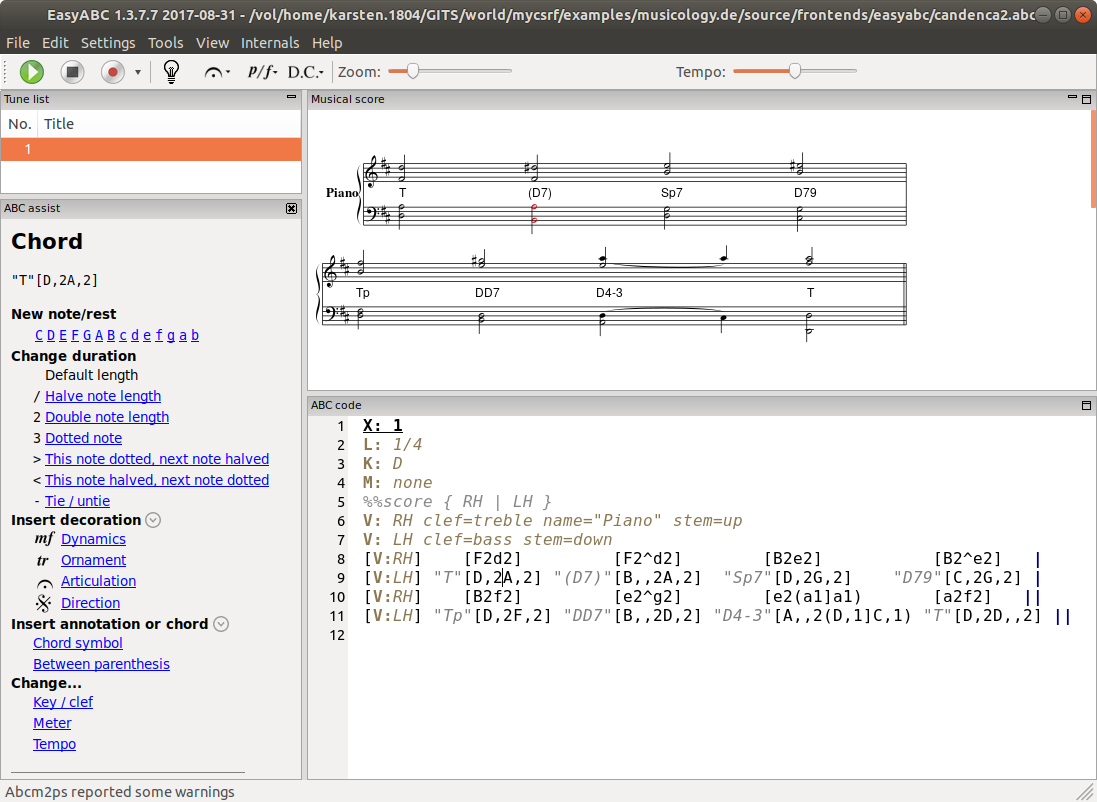
\includegraphics[width=1\textwidth]{frontends/easyabc/easyabc-cadenca2-300dpi.png}
\end{center}


% this is only inserted to eject fault messages in texlipse
%\bibliography{../bib/literature}
